% Options for packages loaded elsewhere
\PassOptionsToPackage{unicode}{hyperref}
\PassOptionsToPackage{hyphens}{url}
\PassOptionsToPackage{dvipsnames,svgnames,x11names}{xcolor}
%
\documentclass[
  letterpaper,
  DIV=11,
  numbers=noendperiod]{scrartcl}

\usepackage{amsmath,amssymb}
\usepackage{iftex}
\ifPDFTeX
  \usepackage[T1]{fontenc}
  \usepackage[utf8]{inputenc}
  \usepackage{textcomp} % provide euro and other symbols
\else % if luatex or xetex
  \usepackage{unicode-math}
  \defaultfontfeatures{Scale=MatchLowercase}
  \defaultfontfeatures[\rmfamily]{Ligatures=TeX,Scale=1}
\fi
\usepackage{lmodern}
\ifPDFTeX\else  
    % xetex/luatex font selection
\fi
% Use upquote if available, for straight quotes in verbatim environments
\IfFileExists{upquote.sty}{\usepackage{upquote}}{}
\IfFileExists{microtype.sty}{% use microtype if available
  \usepackage[]{microtype}
  \UseMicrotypeSet[protrusion]{basicmath} % disable protrusion for tt fonts
}{}
\makeatletter
\@ifundefined{KOMAClassName}{% if non-KOMA class
  \IfFileExists{parskip.sty}{%
    \usepackage{parskip}
  }{% else
    \setlength{\parindent}{0pt}
    \setlength{\parskip}{6pt plus 2pt minus 1pt}}
}{% if KOMA class
  \KOMAoptions{parskip=half}}
\makeatother
\usepackage{xcolor}
\setlength{\emergencystretch}{3em} % prevent overfull lines
\setcounter{secnumdepth}{-\maxdimen} % remove section numbering
% Make \paragraph and \subparagraph free-standing
\ifx\paragraph\undefined\else
  \let\oldparagraph\paragraph
  \renewcommand{\paragraph}[1]{\oldparagraph{#1}\mbox{}}
\fi
\ifx\subparagraph\undefined\else
  \let\oldsubparagraph\subparagraph
  \renewcommand{\subparagraph}[1]{\oldsubparagraph{#1}\mbox{}}
\fi

\usepackage{color}
\usepackage{fancyvrb}
\newcommand{\VerbBar}{|}
\newcommand{\VERB}{\Verb[commandchars=\\\{\}]}
\DefineVerbatimEnvironment{Highlighting}{Verbatim}{commandchars=\\\{\}}
% Add ',fontsize=\small' for more characters per line
\usepackage{framed}
\definecolor{shadecolor}{RGB}{241,243,245}
\newenvironment{Shaded}{\begin{snugshade}}{\end{snugshade}}
\newcommand{\AlertTok}[1]{\textcolor[rgb]{0.68,0.00,0.00}{#1}}
\newcommand{\AnnotationTok}[1]{\textcolor[rgb]{0.37,0.37,0.37}{#1}}
\newcommand{\AttributeTok}[1]{\textcolor[rgb]{0.40,0.45,0.13}{#1}}
\newcommand{\BaseNTok}[1]{\textcolor[rgb]{0.68,0.00,0.00}{#1}}
\newcommand{\BuiltInTok}[1]{\textcolor[rgb]{0.00,0.23,0.31}{#1}}
\newcommand{\CharTok}[1]{\textcolor[rgb]{0.13,0.47,0.30}{#1}}
\newcommand{\CommentTok}[1]{\textcolor[rgb]{0.37,0.37,0.37}{#1}}
\newcommand{\CommentVarTok}[1]{\textcolor[rgb]{0.37,0.37,0.37}{\textit{#1}}}
\newcommand{\ConstantTok}[1]{\textcolor[rgb]{0.56,0.35,0.01}{#1}}
\newcommand{\ControlFlowTok}[1]{\textcolor[rgb]{0.00,0.23,0.31}{#1}}
\newcommand{\DataTypeTok}[1]{\textcolor[rgb]{0.68,0.00,0.00}{#1}}
\newcommand{\DecValTok}[1]{\textcolor[rgb]{0.68,0.00,0.00}{#1}}
\newcommand{\DocumentationTok}[1]{\textcolor[rgb]{0.37,0.37,0.37}{\textit{#1}}}
\newcommand{\ErrorTok}[1]{\textcolor[rgb]{0.68,0.00,0.00}{#1}}
\newcommand{\ExtensionTok}[1]{\textcolor[rgb]{0.00,0.23,0.31}{#1}}
\newcommand{\FloatTok}[1]{\textcolor[rgb]{0.68,0.00,0.00}{#1}}
\newcommand{\FunctionTok}[1]{\textcolor[rgb]{0.28,0.35,0.67}{#1}}
\newcommand{\ImportTok}[1]{\textcolor[rgb]{0.00,0.46,0.62}{#1}}
\newcommand{\InformationTok}[1]{\textcolor[rgb]{0.37,0.37,0.37}{#1}}
\newcommand{\KeywordTok}[1]{\textcolor[rgb]{0.00,0.23,0.31}{#1}}
\newcommand{\NormalTok}[1]{\textcolor[rgb]{0.00,0.23,0.31}{#1}}
\newcommand{\OperatorTok}[1]{\textcolor[rgb]{0.37,0.37,0.37}{#1}}
\newcommand{\OtherTok}[1]{\textcolor[rgb]{0.00,0.23,0.31}{#1}}
\newcommand{\PreprocessorTok}[1]{\textcolor[rgb]{0.68,0.00,0.00}{#1}}
\newcommand{\RegionMarkerTok}[1]{\textcolor[rgb]{0.00,0.23,0.31}{#1}}
\newcommand{\SpecialCharTok}[1]{\textcolor[rgb]{0.37,0.37,0.37}{#1}}
\newcommand{\SpecialStringTok}[1]{\textcolor[rgb]{0.13,0.47,0.30}{#1}}
\newcommand{\StringTok}[1]{\textcolor[rgb]{0.13,0.47,0.30}{#1}}
\newcommand{\VariableTok}[1]{\textcolor[rgb]{0.07,0.07,0.07}{#1}}
\newcommand{\VerbatimStringTok}[1]{\textcolor[rgb]{0.13,0.47,0.30}{#1}}
\newcommand{\WarningTok}[1]{\textcolor[rgb]{0.37,0.37,0.37}{\textit{#1}}}

\providecommand{\tightlist}{%
  \setlength{\itemsep}{0pt}\setlength{\parskip}{0pt}}\usepackage{longtable,booktabs,array}
\usepackage{calc} % for calculating minipage widths
% Correct order of tables after \paragraph or \subparagraph
\usepackage{etoolbox}
\makeatletter
\patchcmd\longtable{\par}{\if@noskipsec\mbox{}\fi\par}{}{}
\makeatother
% Allow footnotes in longtable head/foot
\IfFileExists{footnotehyper.sty}{\usepackage{footnotehyper}}{\usepackage{footnote}}
\makesavenoteenv{longtable}
\usepackage{graphicx}
\makeatletter
\def\maxwidth{\ifdim\Gin@nat@width>\linewidth\linewidth\else\Gin@nat@width\fi}
\def\maxheight{\ifdim\Gin@nat@height>\textheight\textheight\else\Gin@nat@height\fi}
\makeatother
% Scale images if necessary, so that they will not overflow the page
% margins by default, and it is still possible to overwrite the defaults
% using explicit options in \includegraphics[width, height, ...]{}
\setkeys{Gin}{width=\maxwidth,height=\maxheight,keepaspectratio}
% Set default figure placement to htbp
\makeatletter
\def\fps@figure{htbp}
\makeatother
% definitions for citeproc citations
\NewDocumentCommand\citeproctext{}{}
\NewDocumentCommand\citeproc{mm}{%
  \begingroup\def\citeproctext{#2}\cite{#1}\endgroup}
\makeatletter
 % allow citations to break across lines
 \let\@cite@ofmt\@firstofone
 % avoid brackets around text for \cite:
 \def\@biblabel#1{}
 \def\@cite#1#2{{#1\if@tempswa , #2\fi}}
\makeatother
\newlength{\cslhangindent}
\setlength{\cslhangindent}{1.5em}
\newlength{\csllabelwidth}
\setlength{\csllabelwidth}{3em}
\newenvironment{CSLReferences}[2] % #1 hanging-indent, #2 entry-spacing
 {\begin{list}{}{%
  \setlength{\itemindent}{0pt}
  \setlength{\leftmargin}{0pt}
  \setlength{\parsep}{0pt}
  % turn on hanging indent if param 1 is 1
  \ifodd #1
   \setlength{\leftmargin}{\cslhangindent}
   \setlength{\itemindent}{-1\cslhangindent}
  \fi
  % set entry spacing
  \setlength{\itemsep}{#2\baselineskip}}}
 {\end{list}}
\usepackage{calc}
\newcommand{\CSLBlock}[1]{\hfill\break\parbox[t]{\linewidth}{\strut\ignorespaces#1\strut}}
\newcommand{\CSLLeftMargin}[1]{\parbox[t]{\csllabelwidth}{\strut#1\strut}}
\newcommand{\CSLRightInline}[1]{\parbox[t]{\linewidth - \csllabelwidth}{\strut#1\strut}}
\newcommand{\CSLIndent}[1]{\hspace{\cslhangindent}#1}

\KOMAoption{captions}{tableheading}
\makeatletter
\@ifpackageloaded{tcolorbox}{}{\usepackage[skins,breakable]{tcolorbox}}
\@ifpackageloaded{fontawesome5}{}{\usepackage{fontawesome5}}
\definecolor{quarto-callout-color}{HTML}{909090}
\definecolor{quarto-callout-note-color}{HTML}{0758E5}
\definecolor{quarto-callout-important-color}{HTML}{CC1914}
\definecolor{quarto-callout-warning-color}{HTML}{EB9113}
\definecolor{quarto-callout-tip-color}{HTML}{00A047}
\definecolor{quarto-callout-caution-color}{HTML}{FC5300}
\definecolor{quarto-callout-color-frame}{HTML}{acacac}
\definecolor{quarto-callout-note-color-frame}{HTML}{4582ec}
\definecolor{quarto-callout-important-color-frame}{HTML}{d9534f}
\definecolor{quarto-callout-warning-color-frame}{HTML}{f0ad4e}
\definecolor{quarto-callout-tip-color-frame}{HTML}{02b875}
\definecolor{quarto-callout-caution-color-frame}{HTML}{fd7e14}
\makeatother
\makeatletter
\@ifpackageloaded{caption}{}{\usepackage{caption}}
\AtBeginDocument{%
\ifdefined\contentsname
  \renewcommand*\contentsname{Table of contents}
\else
  \newcommand\contentsname{Table of contents}
\fi
\ifdefined\listfigurename
  \renewcommand*\listfigurename{List of Figures}
\else
  \newcommand\listfigurename{List of Figures}
\fi
\ifdefined\listtablename
  \renewcommand*\listtablename{List of Tables}
\else
  \newcommand\listtablename{List of Tables}
\fi
\ifdefined\figurename
  \renewcommand*\figurename{Figure}
\else
  \newcommand\figurename{Figure}
\fi
\ifdefined\tablename
  \renewcommand*\tablename{Table}
\else
  \newcommand\tablename{Table}
\fi
}
\@ifpackageloaded{float}{}{\usepackage{float}}
\floatstyle{ruled}
\@ifundefined{c@chapter}{\newfloat{codelisting}{h}{lop}}{\newfloat{codelisting}{h}{lop}[chapter]}
\floatname{codelisting}{Listing}
\newcommand*\listoflistings{\listof{codelisting}{List of Listings}}
\makeatother
\makeatletter
\makeatother
\makeatletter
\@ifpackageloaded{caption}{}{\usepackage{caption}}
\@ifpackageloaded{subcaption}{}{\usepackage{subcaption}}
\makeatother
\ifLuaTeX
  \usepackage{selnolig}  % disable illegal ligatures
\fi
\usepackage{bookmark}

\IfFileExists{xurl.sty}{\usepackage{xurl}}{} % add URL line breaks if available
\urlstyle{same} % disable monospaced font for URLs
\hypersetup{
  pdftitle={U.S. National Park Visit Data (1979-2023) (No Tabs Version)},
  pdfauthor={Melanie Walsh and Os Keyes},
  colorlinks=true,
  linkcolor={blue},
  filecolor={Maroon},
  citecolor={Blue},
  urlcolor={Blue},
  pdfcreator={LaTeX via pandoc}}

\title{U.S. National Park Visit Data (1979-2023) (No Tabs Version)}
\author{Melanie Walsh and Os Keyes}
\date{2024-03-09}

\begin{document}
\maketitle

\begin{tcolorbox}[enhanced jigsaw, bottomrule=.15mm, colback=white, colbacktitle=quarto-callout-warning-color!10!white, coltitle=black, titlerule=0mm, leftrule=.75mm, toprule=.15mm, opacitybacktitle=0.6, colframe=quarto-callout-warning-color-frame, opacityback=0, rightrule=.15mm, breakable, bottomtitle=1mm, toptitle=1mm, title={Find All Materials in ``Guide''}, left=2mm, arc=.35mm]

To access all materials associated with this dataset, be sure to check
the ``Guide'' in the sidebar.

\end{tcolorbox}

\subsection{Introduction}\label{introduction}

This dataset contains the number of visits, per year, to each of the
current
\href{https://en.wikipedia.org/wiki/List_of_national_parks_of_the_United_States\#National_parks}{63
National Parks} administered by the United States National Park Service
(NPS), from 1979 to the present. The NPS also collects visitation and
use data about other park units, such as
\href{(https://www.nps.gov/aboutus/national-park-system.htm)}{national
battlefields, national rivers, and national monuments}. However,
information about other park units is not included in this particular
dataset.

\begin{tcolorbox}[enhanced jigsaw, bottomrule=.15mm, colback=white, colbacktitle=quarto-callout-tip-color!10!white, coltitle=black, titlerule=0mm, leftrule=.75mm, toprule=.15mm, opacitybacktitle=0.6, colframe=quarto-callout-tip-color-frame, opacityback=0, rightrule=.15mm, breakable, bottomtitle=1mm, toptitle=1mm, title={Brief Survey}, left=2mm, arc=.35mm]

If you use our materials in your class or another setting, we would love
to \href{https://forms.gle/yJpQscUH9k9Rn4Qy9}{hear about it}!

\end{tcolorbox}

\begin{Shaded}
\begin{Highlighting}[]
\NormalTok{//|echo: false}
\NormalTok{import \{viewof dataSummaryView, viewof selectedColumns, viewof dataUrl, viewof dataSet, tableContainer, table, viewof tableOptions, tableStyles\} from "ac13d95a907715bf"}
\end{Highlighting}
\end{Shaded}

\begin{Shaded}
\begin{Highlighting}[]
\NormalTok{//|echo: false}
\NormalTok{viewof dataSet}
\NormalTok{viewof dataUrl}
\NormalTok{viewof tableOptions}
\end{Highlighting}
\end{Shaded}

\begin{Shaded}
\begin{Highlighting}[]
\NormalTok{//|echo: false}
\NormalTok{tableContainer}
\end{Highlighting}
\end{Shaded}

\begin{Shaded}
\begin{Highlighting}[]
\NormalTok{//|echo: false}
\NormalTok{//|output: false}
\NormalTok{table}
\NormalTok{html\textasciigrave{}\textless{}link href=\textquotesingle{}https://unpkg.com/tabulator{-}tables@5.3.1/dist/css/tabulator.min.css\textquotesingle{} rel=\textquotesingle{}stylesheet\textquotesingle{} /\textgreater{}}
\NormalTok{tabulator.min.css\textasciigrave{}}
\end{Highlighting}
\end{Shaded}

\begin{Shaded}
\begin{Highlighting}[]
\NormalTok{//|echo: false}
\NormalTok{viewof selectedColumns}
\NormalTok{viewof dataSummaryView}
\end{Highlighting}
\end{Shaded}

\begin{tcolorbox}[enhanced jigsaw, bottomrule=.15mm, colback=white, colbacktitle=quarto-callout-tip-color!10!white, coltitle=black, titlerule=0mm, leftrule=.75mm, toprule=.15mm, opacitybacktitle=0.6, colframe=quarto-callout-tip-color-frame, opacityback=0, rightrule=.15mm, breakable, bottomtitle=1mm, toptitle=1mm, title={Creative Commons License}, left=2mm, arc=.35mm]

This work is licensed under CC BY 4.0

\end{tcolorbox}

The National Park datasets included on this website are drawn from data
published by the National Park Service. Most (but not all) of the
contextual information included here draws from material published by
the National Park Service, as well. However, the original data is made
available in an \href{https://irma.nps.gov/Stats/}{NPS data portal} that
is relatively hard to find, and the documentation is distributed across
many different web pages, PDFs, and other documents. Thus, we believe it
is valuable to publish a synthesized verison of the documentation here
and to tell a narrative version of how this data came to be, what its
flaws are, and why it matters.

The datasets were curated and published by Melanie Walsh, and the data
essay was written by Os Keyes and Melanie Walsh.

\subsection{History}\label{history}

The very first National Park ---~Yellowstone National Park, in Wyoming
---~was signed into law by President Ulysses S. Grant in 1872. A handful
of other parks ---~Sequoia, Yosemite, Mt. Rainier, Crater Lake~---
joined the system in the next several decades. While the National Parks
were originally created to protect precious, beautiful lands and to make
them accessible to the public --- a noble goal --- it's important to
remember that these lands were taken, often forcibly, from Native
American people who already owned, lived, and worked on them (Beauchamp
2020). Today, there are still calls for the NPS to
\href{https://www.theatlantic.com/magazine/archive/2021/05/return-the-national-parks-to-the-tribes/618395/}{return
the lands of the National Parks to Indigenous people.}

Scholars have similarly shown that early conservation movements, which
spurred the development of the National Parks, were troublingly
intertwined with racism and eugenics movements (Beauchamp 2020). These
prejudiced origins, combined with continuing forms of environmental
racism, have contributed to the marginalization of people of color and
other minorities in the parks; research has shown that white people
visit the parks much more than other demographic groups(Weber and
Sultana 2013; Alba et al. 2022; Floyd and Johnson 2002). The National
Parks are not equally accessible to everyone in the same way, and these
exclusions shape the park visitation data even before it's counted.

Visit counting, according to the NPS, started a long time ago ---
\href{https://www.nps.gov/subjects/socialscience/visitor-use-statistics.htm}{as
early as 1904} (more than 10 years before the National Park Service
itself was officially created). However, at this time, their data
collection methods were mostly
\href{https://www.nps.gov/subjects/socialscience/visitor-use-statistics.htm}{informal,
inconsistent, and low-tech}. But over the next century, the NPS worked
hard to make their methods more reliable, consistent, and
technologically advanced.

A big catalyst for the NPS getting serious about data collection was a
new law. In 1965, the U.S. Congress passed
\href{https://www.everycrsreport.com/reports/RL33531.html}{The Land and
Water Conservation Fund Act of 1965}. This act created a new source of
government money specifically dedicated to protecting natural resources
(i.e.~to buying up more land and water so that condo developers couldn't
do it first) and to expanding outdoor recreation infrastructure in the
U.S.

Because this act stipulated that the amount of money allocated to each
area should be
\href{https://www.nps.gov/subjects/socialscience/statistics-history.htm}{``proportional
to visitor use,''} the NPS buckled down on counting visitor use. Over
the next twenty years, they accordingly
\href{https://www.nps.gov/subjects/socialscience/statistics-history.htm}{``developed
and institutionalized a formal system for collecting, compiling and
reporting visitor use data.''}

While today's National Park data collection system is more formal and
sophisticated than the one that the NPS used in 1904, there are still
many inconsistencies, flaws, and limitations. These shortcomings are
largely unavoidable. Think about it. Would it be possible to record
*every* *single* *visit* to *every* *single* National Park\ldots{}
*ever*? We're talking about 60 different parks and dozens of different
geographic areas (mountains, volcanoes, deserts, canyons, wetlands,
forests, islands, and more); over 40 years; in countless changing
weather conditions; amidst various economic fluctuation and National
Park staff support and funding; and hundreds of millions of people who
are walking, hiking, backpacking, driving, boating, biking, skiing, and
more. It's just not possible. However, we believe this data is useful to
study precisely for this reason: because it helps demonstrate that
\textbf{\emph{data never reflects reality precisely}}.

And yet the National Park visit data also demonstrates why collecting
and analyzing data, even if it is flawed and approximate, is sometimes
worthwhile --- if (big if) you fully understand the data's flaws,
limitations, and history, and if you incorporate these considerations
into all subsequent analyses, interpretations, and takeaways.

\subsection{Where did the data come from? Who collected
it?}\label{where-did-the-data-come-from-who-collected-it}

The National Park data on this website was originally organized and
published by the
\href{https://www.nps.gov/subjects/socialscience/visitor-use-statistics.htm}{NPS
Social Science Program}, a specific program tasked with coordinating
visitor statistics across the parks. Thousands of staff members across
all 63 parks were also involved in the data collection process.

The original data was made available through the NPS's
\href{https://irma.nps.gov/Stats/}{Visitor Use Statistics data portal}.
Through this portal, you can generate reports and download data for
\href{https://irma.nps.gov/Stats/Reports/National}{many different park
visitation categories} and time periods~---~at both national and
individual park levels. To download the data included here, we first
selected \href{https://irma.nps.gov/Stats/Reports/National}{``National
Reports''} in the data portal, and we then selected the
\href{https://irma.nps.gov/Stats/SSRSReports/National\%20Reports/Query\%20Builder\%20for\%20Public\%20Use\%20Statistics\%20(1979\%20-\%20Last\%20Calendar\%20Year)}{``Query
Builder for Public Use Statistics (1979 - Last Calendar Year)''} report
type.

\begin{figure}

\centering{

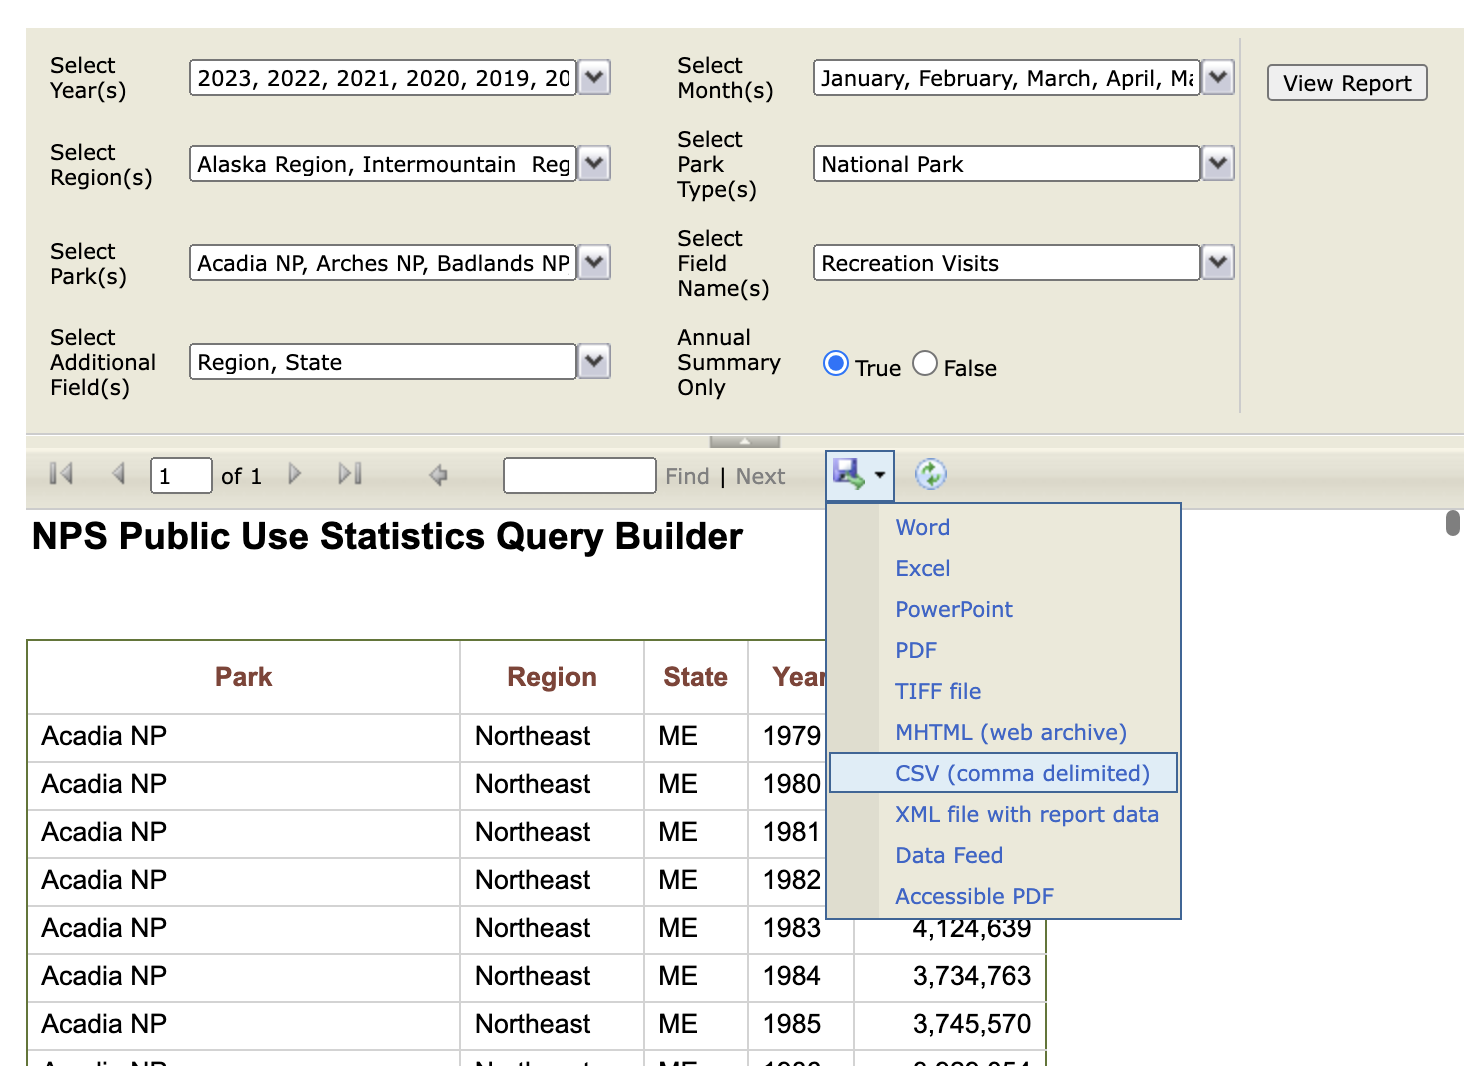
\includegraphics[width=0.9\textwidth,height=\textheight]{images/query-builder-csv-screenshot.png}

}

\caption{\label{fig-query-builder}Selections for National Park visit
data generated with
\href{https://irma.nps.gov/Stats/SSRSReports/National\%20Reports/Query\%20Builder\%20for\%20Public\%20Use\%20Statistics\%20(1979\%20-\%20Last\%20Calendar\%20Year)}{``Query
Builder for Public Use Statistics (1979 - Last Calendar Year)''}}

\end{figure}%

For ``Park Types,'' we selected only ``National Parks''; for ``Years,''
we selected all possible years (1979-2023); for ``Regions,'' we selected
all possible regions; for ``Field Type,'' we selected only ``Recreation
Visits'' (excluding ``NonRecreation Visits,'''' ``Recreation Hours,''
``NonRecreation Hours,'' ``Concessioner Lodging,'' ``Concessioner
Camping,'' ``Tent Campers,'' ``RV Campers,'' ``Backcountry Campers,''
``NonRecreation Overnight Stays,'' and ``Miscellaneous Overnight
Stays''); for ``Additional Fields,'' we selected ``State'' and
``Region''. We also selected the option of viewing the report as an
annual summary of visit counts (as opposed to monthly visit counts).

If you choose to download this report as a CSV file, it will
unfortunately not look exactly like the report pictured in
Figure~\ref{fig-query-builder}; instead, the CSV will include all visit
and use types, and it will include visit/use information by month rather
than aggregated by year. When I have compiled this data to share with my
students in the past, I have sometimes downloaded the CSV file and then
removed the columns that I'm not interested in and aggregated the data
by year programatically. In other cases, I have simply copied and pasted
the annual summary report into a CSV file.

In either case, it is usually necessary to explicitly transform the
format of the ``RecreationVisits'' column into a number and to remove
the commas that separate the numbers by thousands (a transformation that
you can do with spreadsheet applications like Excel or Google Sheets or
with a programming language) Finally, we published the data to this
project's GitHub repository for easier storage and access.

\subsection{Why was the data collected? How is the data
used?}\label{why-was-the-data-collected-how-is-the-data-used}

The NPS collects visit data partly because the government requires it,
as we've already discussed. But the NPS also uses the visit data for
other internal purposes ---~to determine which parks need more staff
members and programming, which hiking trails need more maintenance, or
which visitor centers need more bathrooms.

The visit data also helps the communities and businesses surrounding the
parks understand how they can best provide and share resources, like
emergency vehicles, sanitation, and water. If millions more hikers
started to come to Mt. Rainier, for example, that would be a very
important thing for the surrounding community to know. To consider just
one consequence of this increase, those hikers would likely need more
ambulance trips and rescue helicopters, and you wouldn't want visitors
to the local National Park booking up all the emergency vehicles in
town.

\begin{figure}

\centering{

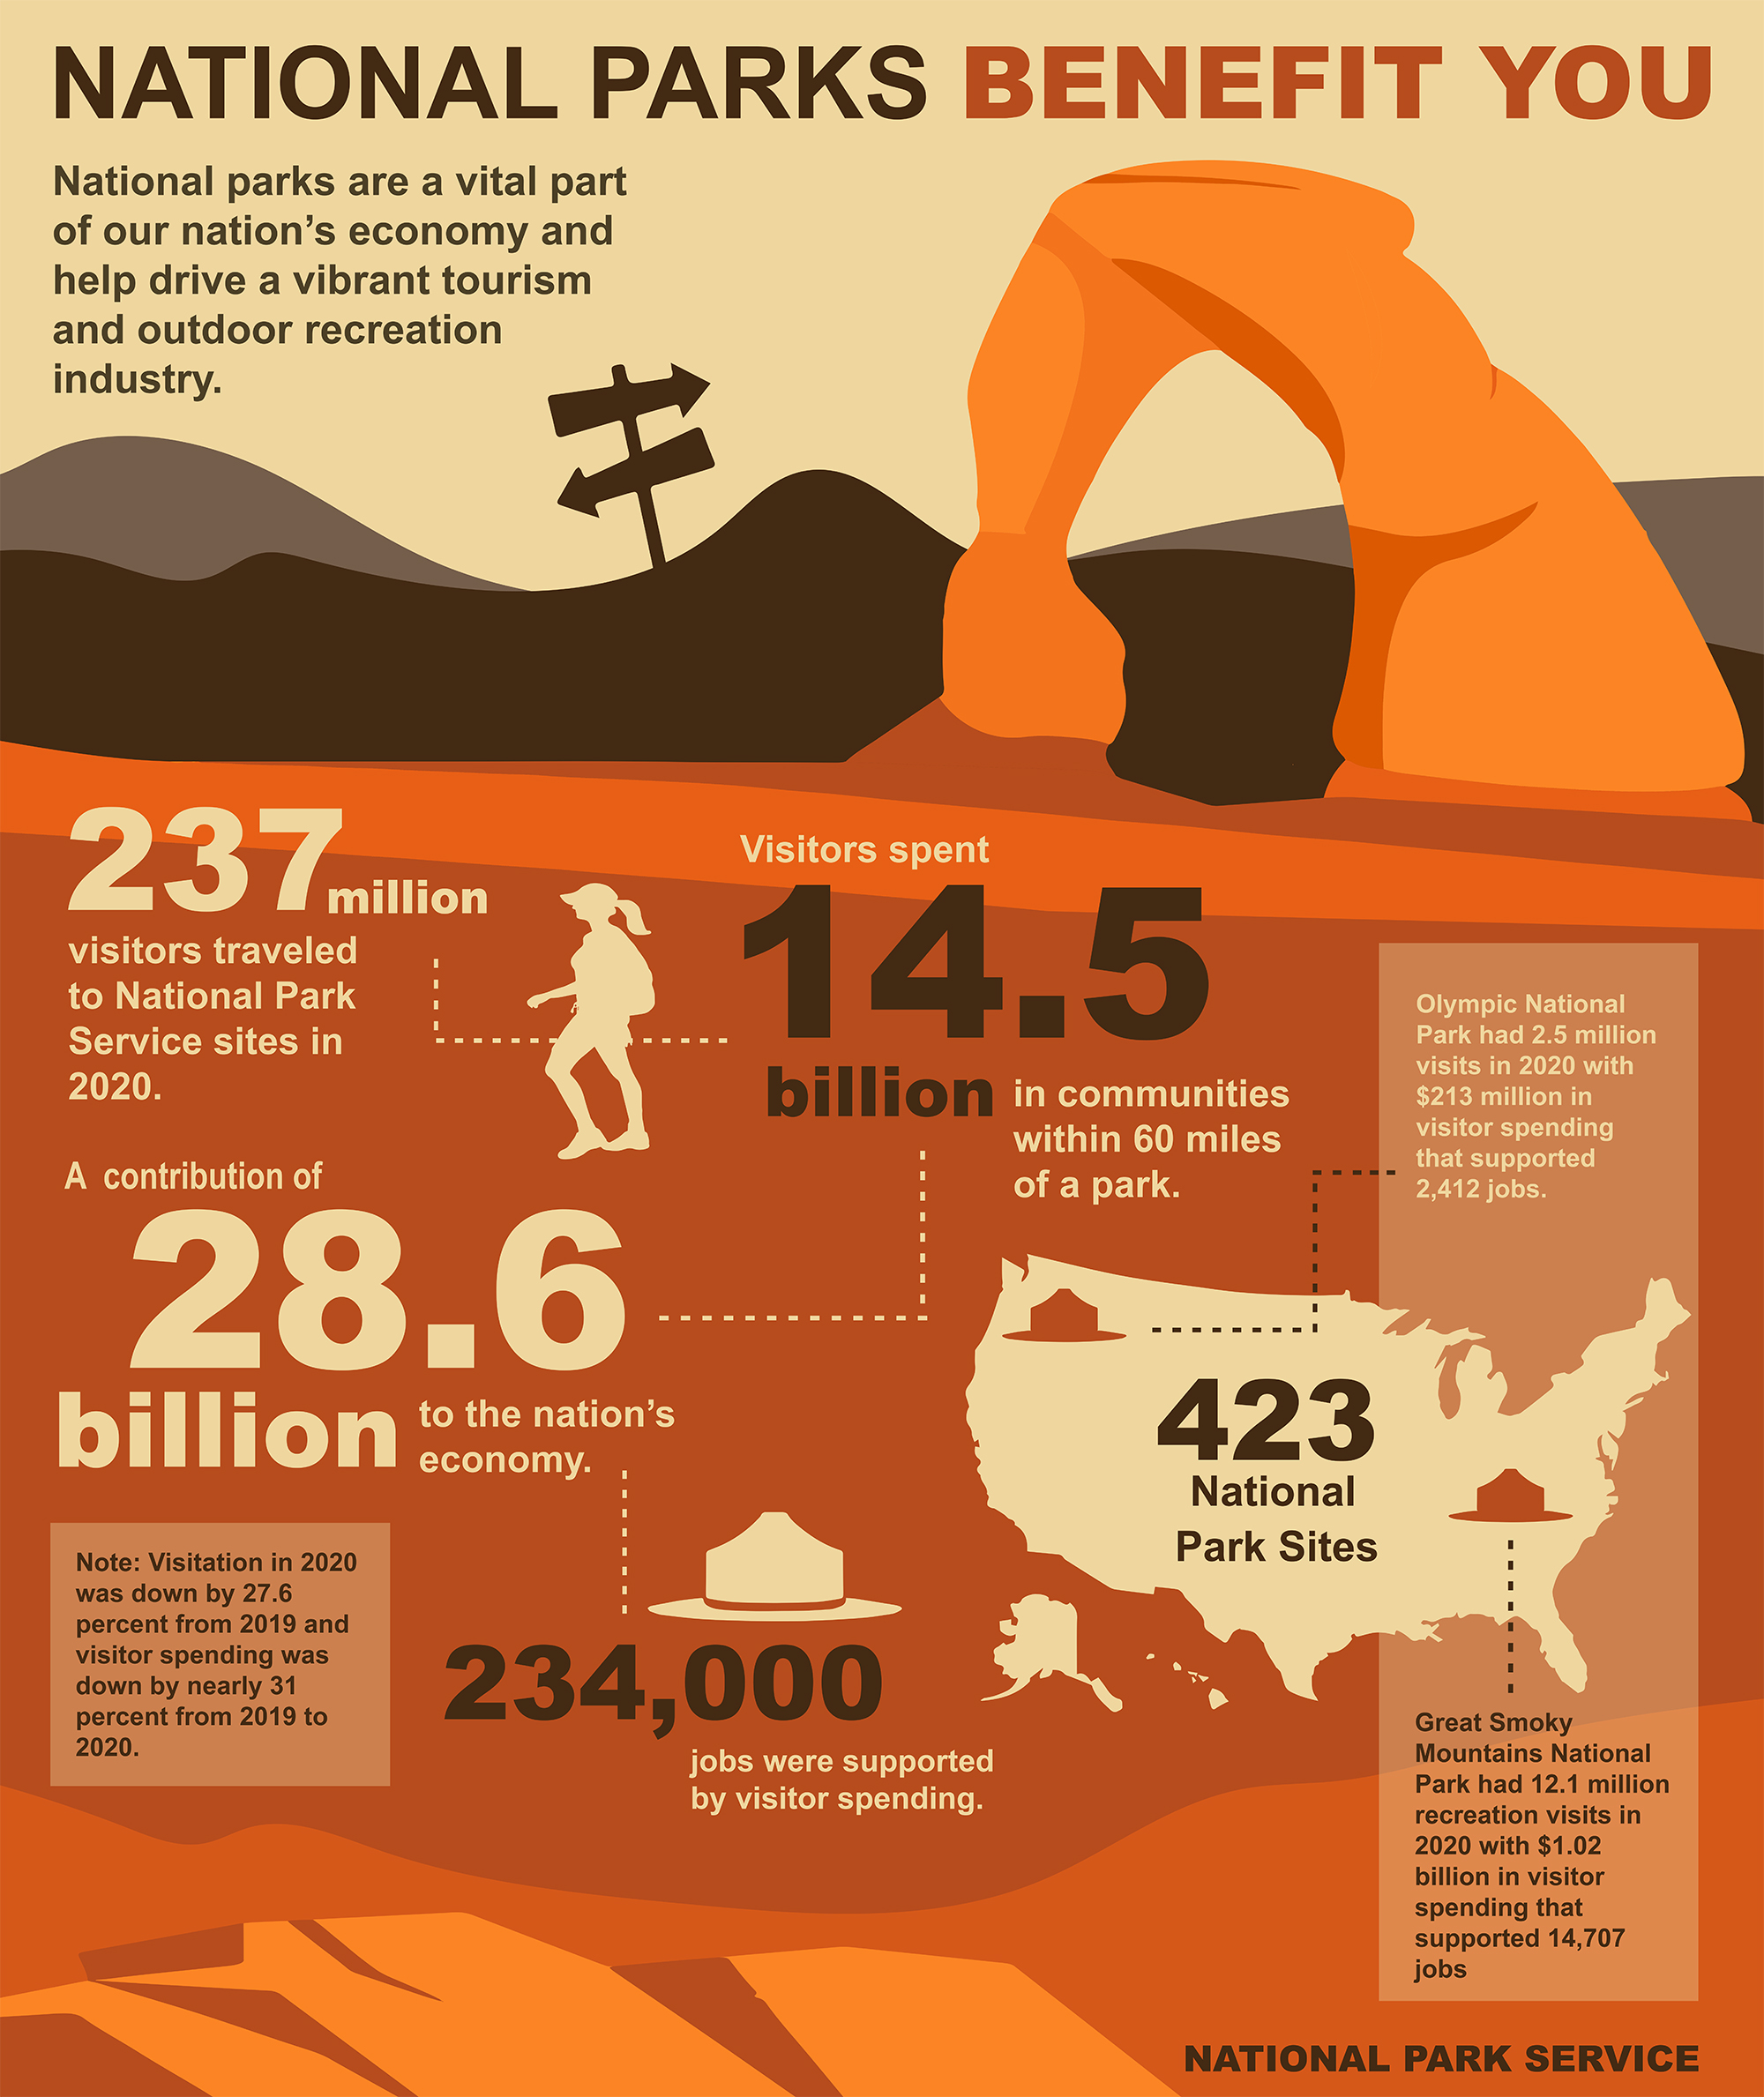
\includegraphics[width=0.9\textwidth,height=\textheight]{data-essay_files/mediabag/ECONOMIC-2020.jpg}

}

\caption{\label{fig-economic-benefit}2021 report on NPS economic impact
// \href{https://www.nps.gov/orgs/1207/vse2020.htm}{Graphic by NPS}}

\end{figure}%

The visitation data also helps the NPS estimate the beneficial
impact---economic and otherwise---that the parks have on nearby
communities and the nation at large (Figure~\ref{fig-economic-benefit}).
These estimations are important because they help the parks advocate for
more funding, support, and attention.

The data is also frequently reported on by journalists, who use it to
highlight the most popular parks and noteworthy visitation records, as
well as to point their readers to parks where they might be able to find
some peace and quiet (see articles in
\href{https://www.thrillist.com/news/nation/most-visited-national-parks-ranked-nps}{Thrillist},
\href{https://www.smithsonianmag.com/smart-news/most-and-least-popular-national-parks-2023-180983850/}{Smithsonian},
and
\href{https://www.cnn.com/travel/article/most-visited-us-national-park-sites-2022/index.html}{CNN}).

\subsection{What's in the data? What ``counts'' as a
visit?}\label{whats-in-the-data-what-counts-as-a-visit}

Now that we know how the data is used, let's dive into the data itself.
What's actually in this dataset, and what ``counts'' as a visit?

To get started, let's load the dataset and examine a random sample of
rows.

\begin{Shaded}
\begin{Highlighting}[]
\CommentTok{\# https://statsandr.com/blog/an{-}efficient{-}way{-}to{-}install{-}and{-}load{-}r{-}packages/}

\CommentTok{\# Load the dplyr package}
\FunctionTok{library}\NormalTok{(dplyr, }\AttributeTok{warn =} \ConstantTok{FALSE}\NormalTok{)}

\CommentTok{\# Load National Park Visitation data}
\NormalTok{np\_data }\OtherTok{\textless{}{-}} \FunctionTok{read.csv}\NormalTok{(}\StringTok{"https://raw.githubusercontent.com/melaniewalsh/responsible{-}datasets{-}in{-}context/main/datasets/national{-}parks/US{-}National{-}Parks\_RecreationVisits\_1979{-}2023.csv"}\NormalTok{, }\AttributeTok{stringsAsFactors =} \ConstantTok{FALSE}\NormalTok{)}

\DocumentationTok{\#\# Look at the structure of the dataset, randomly sample 10 rows}
\NormalTok{np\_data }\SpecialCharTok{\%\textgreater{}\%} \FunctionTok{slice\_sample}\NormalTok{(}\AttributeTok{n =} \DecValTok{10}\NormalTok{)}
\end{Highlighting}
\end{Shaded}

\begin{longtable}[]{@{}lllrr@{}}
\toprule\noalign{}
ParkName & Region & State & Year & RecreationVisits \\
\midrule\noalign{}
\endhead
\bottomrule\noalign{}
\endlastfoot
Glacier Bay NP \& PRES & Alaska & AK & 2012 & 454337 \\
Zion NP & Intermountain & UT & 2007 & 2657281 \\
Redwood NP & Pacific West & CA & 2004 & 392029 \\
Indiana Dunes NP & Midwest & IN & 1989 & 1791902 \\
Hot Springs NP & Midwest & AR & 1980 & 1160588 \\
Olympic NP & Pacific West & WA & 1999 & 3364266 \\
Badlands NP & Midwest & SD & 2000 & 1105824 \\
Wind Cave NP & Midwest & SD & 2014 & 547022 \\
Sequoia NP & Pacific West & CA & 2008 & 930011 \\
Hot Springs NP & Midwest & AR & 2018 & 1506887 \\
\end{longtable}

Here we see five columns -- ``ParkName'', ``Region'', ``State'',
``Year'', and ``RecreationVisits.'' The first four are pretty
self-explanatory, but why is the fifth labelled ``RecreationVisits''
rather than ``Visits'' or ``Visitors''?

It turns out that the NPS distinguishes between \emph{kinds} of visits
to their parks. There are ``recreation'' visits ---~when people are
visiting the parks for fun, vacation, exercise, etc. --- and there are
``non-recreation'' visits ---~when people are visiting the parks for
other reasons. For example, some people need to travel \emph{through}
the parks, either because a highway runs through the park, or because
they live on ``inholdings'' (private property that is surrounded by a
National Park on all sides). Other people are visiting the parks because
they have actual business to conduct in the parks.

Here's a
\href{https://www.nps.gov/subjects/socialscience/nps-visitor-use-statistics-definitions.htm}{full
list of ``reportable non-recreation'' visits}according to the NPS:

\begin{quote}
\begin{itemize}
\tightlist
\item
  Persons going to and from inholdings across significant parts of park
  land;
\item
  Commuter and other traffic using NPS-administered roads or waterways
  through a park for their convenience;
\item
  Trades-people with business in the park;
\item
  Any civilian activity a part of or incidental to the pursuit of a
  gainful occupation (e.g., guides);
\item
  Government personnel (other than NPS employees) with business in the
  park;
\item
  Citizens using NPS buildings for civic or local government business,
  or attending public hearings;
\item
  Outside research activities (visits and overnights) if independent of
  NPS legislated interests (e.g.~meteorological research).
\end{itemize}
\end{quote}

What this means is that ``recreation visit'' counts leave out a lot of
people. This is worth thinking about when we evaluate what the numbers
mean, and how the NPS achieves them (which we'll discuss more below).

It also means that they're not counting individual people. This data
doesn't tell us anything \emph{about} the people who are visiting.

(Note: The Pine Ridge Indian Reservation in South Dakota is located
inside Badlands National Park (the visitor center is on the
reservation), which could be worth discussing here.)

\subsection{How was the data
collected?}\label{how-was-the-data-collected}

So how does the NPS actually count these recreation visits? Take a
moment and see if you come up with a few guesses\ldots{}

It turns out that each park counts visits differently. And at many
parks, \emph{each entrance} at each park even counts visits differently.

If you go to the \href{https://irma.nps.gov/Stats/Reports/Park}{``Park
Reports''} tab in the NPS Data Portal, you can look up an individual
park and download a PDF file called ``Visitor Use Counting Procedures,''
which details exactly what procedures they use to count visits at this
park. Most of the parks have several PDFs because their counting
procedures have changed many times over the years!

To count visits, most parks use a combination of automatic traffic
counters and manual counting---that is, staff members who use their
eyeballs to literally count the number of people arriving by foot, bike,
bus, cross-country skis, snowmobile, boat, canoe, etc. Perhaps most
interesting, they usually take those counts and then apply a
specifically designed mathematical formula to arrive at the most
accurate estimate of number of recreation visits --- adding,
subtracting, and multiplying the counts based on a variety of factors,
such as the season or the entrance (e.g.~assuming that more people would
likely be arriving in a car in the summer months at the most popular
gate than in the winter months at the least popular gate) or how many
non-recreation visits they expect are a confounding factor.

For example, at Everglades National Park, at the Shark Valley Entrance,
there is a pneumatic tube traffic counter that counts the number of cars
that pass over it. The staff members then apply different mathematical
operations to this number in order to arrive at what they think is the
most accurate estimate of recreation visits:

\begin{quote}
The traffic count is divided by 2 to account for entry and exit. The
adjusted traffic count is reduced by the number of buses, the number of
bicycles counted when the entrance station is open, 127 bicycles per
month to account for after-hours use, and by 200 non-recreation vehicles
per month October through May and 100 non-recreation vehicles per month
June through September. The traffic count is further reduced by 350
non-reportable (NPS) vehicles per month. The reduced count is multiplied
by 2.17 persons per vehicle.
\end{quote}

What's more, the devices that the NPS uses to count visits, like
pneumatic tube counters or induction loop counters (magnetised coils of
wire that are installed under a road, and that ``trip'' when a vehicle
passes over them) sometimes break.

\begin{figure}[H]

{\centering \includegraphics[width=3.125in,height=\textheight]{data-essay_files/mediabag/Metrocount_vehicle_c.jpg-20110223182337}

}

\caption{An example of a pneumatic tube traffic counter, installed above
the road}

\end{figure}%%
\begin{figure}[H]

{\centering \includegraphics[width=3.125in,height=\textheight]{data-essay_files/mediabag/Inductance_detectors.jpg}

}

\caption{An example of an induction loop, installed beneath a road
(making it harder to detect when it breaks!)}

\end{figure}%

For example,
\href{https://irma.nps.gov/Stats/SSRSReports/Park\%20Specific\%20Reports/Monthly\%20Visitation\%20Comments\%20By\%20Park?Park=CRLA}{according
to the NPS data logs}, the induction loop counter at one of the main
entrances at Crater Lakes National Park broke in 2012 and wasn't
repaired for at least a year:

\begin{quote}
2/1/2012 \textbar{} The Traffic Counter at Annie Springs Entrance
Station was not functioning properly and therefore we have a count of
zero.
\end{quote}

\begin{quote}
3/1/2012 \textbar{} Broken counter at Annie Springs Entrance, unable to
record numbers.
\end{quote}

\begin{quote}
4/1/2012 \textbar{} Traffic counter was broken for the beginning of the
month and may have low numbers.
\end{quote}

\begin{quote}
10/1/2012 \textbar{} Counts estimated by Butch
\end{quote}

\begin{quote}
11/1/2012 \textbar{} TRAFFIC COUNT AT ANNIE SPRINGS ENTRANCE NOT
AVAILIBLE
\end{quote}

\begin{quote}
12/1/2012 \textbar{} TRAFFIC COUNT AT ANNIE SPRINGS ENTRANCE NOT
AVAILIBLE
\end{quote}

\begin{quote}
1/1/2013 \textbar{} Traffic count at Annie Springs estimated.
\end{quote}

\begin{quote}
2/1/2013 \textbar{} Traffic count at Annie Springs estimated.
\end{quote}

You can see a similar, but more severe, example at Carlsbad Caverns
National Park, where it appears that visits have been declining since
around 2019:

\begin{Shaded}
\begin{Highlighting}[]
\CommentTok{\# Load the "ggplot2" package (which we\textquotesingle{}ll be using a lot more)}
\FunctionTok{library}\NormalTok{(ggplot2)}

\CommentTok{\# Let\textquotesingle{}s also load "ggthemes", which let\textquotesingle{}s us use colorblind{-}compatible palettes. When we\textquotesingle{}ve only got one line, this will just be black.}
\FunctionTok{library}\NormalTok{(ggthemes)}

\CommentTok{\# And specify the colorblind palette}
\NormalTok{cb\_palette }\OtherTok{\textless{}{-}} \FunctionTok{colorblind\_pal}\NormalTok{()(}\DecValTok{8}\NormalTok{)}

\CommentTok{\# Turn off scientific notation}
\FunctionTok{options}\NormalTok{(}\AttributeTok{scipen =} \DecValTok{999}\NormalTok{)}

\CommentTok{\# Filter down to Carlsbad Caverns National Park}
\NormalTok{carlsbad\_data }\OtherTok{\textless{}{-}}\NormalTok{ np\_data }\SpecialCharTok{\%\textgreater{}\%} \FunctionTok{filter}\NormalTok{(ParkName }\SpecialCharTok{==} \StringTok{"Carlsbad Caverns NP"}\NormalTok{)}

\CommentTok{\# Visualise it}
\FunctionTok{ggplot}\NormalTok{(}\AttributeTok{data =}\NormalTok{ carlsbad\_data) }\SpecialCharTok{+} 
  \FunctionTok{geom\_line}\NormalTok{(}\FunctionTok{aes}\NormalTok{(}\AttributeTok{x =}\NormalTok{ Year, }\AttributeTok{y =}\NormalTok{ RecreationVisits), }\AttributeTok{color =}\NormalTok{ cb\_palette[}\DecValTok{2}\NormalTok{]) }\SpecialCharTok{+} 
  \FunctionTok{labs}\NormalTok{(}\AttributeTok{title =} \StringTok{"Carlsbad Caverns National Park Visits (1979 {-} Present)"}\NormalTok{)}
\end{Highlighting}
\end{Shaded}

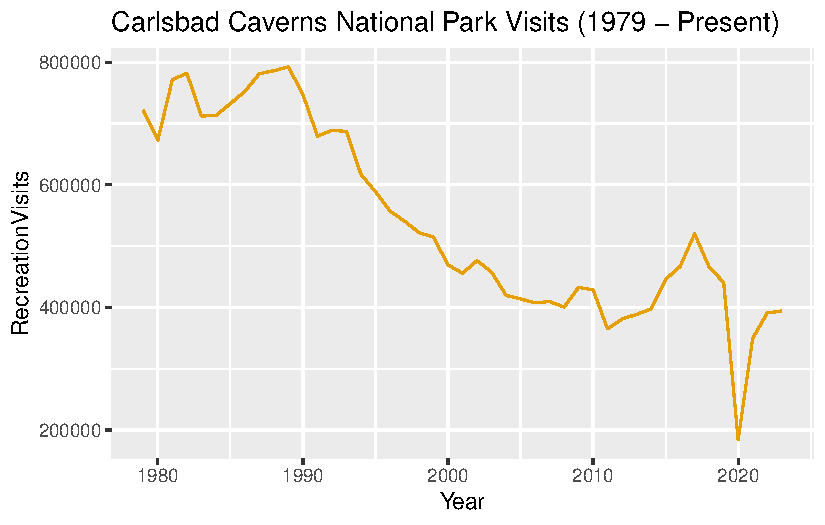
\includegraphics{data-essay_files/figure-pdf/unnamed-chunk-7-1.pdf}

This decline may, in part, be due to the COVID-19 pandemic.

But the NPS logs also show that the main induction loop counter at
Carlsbad Caverns
\href{https://irma.nps.gov/Stats/SSRSReports/Park\%20Specific\%20Reports/Monthly\%20Visitation\%20Comments\%20By\%20Park?Park=CAVE}{broke
in 2019 and has remained broken for multiple years}:

\begin{quote}
9/1/2019 \textbar{} Traffic counter apparently has been broken since
July. Traffic counts are estimated.
\end{quote}

\begin{quote}
4/1/2020 \textbar{} Main road traffic counter is broken, I have
estimated the count.
\end{quote}

\begin{quote}
12/1/2020 \textbar{} Corona virus closure that began in November ended
on December 4th. Main road traffic counter remains broken.Possible
problem with Loop Road counter.
\end{quote}

\begin{quote}
4/1/2022 Main road traffic counter remains broken. Rattlesnake Springs
traffic counter seems to be off, I will henceforth provide estimates.
\end{quote}

\begin{quote}
9/1/2023 \textbar{} Loop Road and backcountry closed due to flood
damage. Slaughter Canyon Cave remains closed Traffic counter on main
road remains broken.
\end{quote}

\begin{tcolorbox}[enhanced jigsaw, bottomrule=.15mm, colback=white, colbacktitle=quarto-callout-tip-color!10!white, coltitle=black, titlerule=0mm, leftrule=.75mm, toprule=.15mm, opacitybacktitle=0.6, colframe=quarto-callout-tip-color-frame, opacityback=0, rightrule=.15mm, breakable, bottomtitle=1mm, toptitle=1mm, title=\textcolor{quarto-callout-tip-color}{\faLightbulb}\hspace{0.5em}{Activity 1}, left=2mm, arc=.35mm]

Now that we've talked about how data is collected (and the fragility of
some of those methods), it's a good time to think about how even the
same method, deployed at different places, might be differently
unreliable. For more, see
\href{?tab=discussion-\%26-activities\#activity-1-1}{Activity 1}.

\end{tcolorbox}

\subsection{What data is missing? How is uncertainty
handled?}\label{what-data-is-missing-how-is-uncertainty-handled}

If you filter the data and examine the least visited National Parks
across these many decades, you'll notice that there are some parks that
had \emph{zero} visitors in a given year.

\begin{Shaded}
\begin{Highlighting}[]
\CommentTok{\# Filter for minimum RecVisits}
\NormalTok{least\_visited }\OtherTok{\textless{}{-}}\NormalTok{ np\_data }\SpecialCharTok{\%\textgreater{}\%} \FunctionTok{filter}\NormalTok{(RecreationVisits }\SpecialCharTok{==} \FunctionTok{min}\NormalTok{(RecreationVisits))}

\CommentTok{\# Number of rows for least visited}
\NormalTok{num\_rows }\OtherTok{\textless{}{-}} \FunctionTok{nrow}\NormalTok{(least\_visited)}

\CommentTok{\# Show some of them}
\NormalTok{least\_visited  }\SpecialCharTok{\%\textgreater{}\%} \FunctionTok{slice\_sample}\NormalTok{(}\AttributeTok{n =} \FunctionTok{min}\NormalTok{(}\DecValTok{10}\NormalTok{, num\_rows))}
\end{Highlighting}
\end{Shaded}

\begin{longtable}[]{@{}
  >{\raggedright\arraybackslash}p{(\columnwidth - 8\tabcolsep) * \real{0.4384}}
  >{\raggedright\arraybackslash}p{(\columnwidth - 8\tabcolsep) * \real{0.1781}}
  >{\raggedright\arraybackslash}p{(\columnwidth - 8\tabcolsep) * \real{0.0822}}
  >{\raggedleft\arraybackslash}p{(\columnwidth - 8\tabcolsep) * \real{0.0685}}
  >{\raggedleft\arraybackslash}p{(\columnwidth - 8\tabcolsep) * \real{0.2329}}@{}}
\toprule\noalign{}
\begin{minipage}[b]{\linewidth}\raggedright
ParkName
\end{minipage} & \begin{minipage}[b]{\linewidth}\raggedright
Region
\end{minipage} & \begin{minipage}[b]{\linewidth}\raggedright
State
\end{minipage} & \begin{minipage}[b]{\linewidth}\raggedleft
Year
\end{minipage} & \begin{minipage}[b]{\linewidth}\raggedleft
RecreationVisits
\end{minipage} \\
\midrule\noalign{}
\endhead
\bottomrule\noalign{}
\endlastfoot
National Park of American Samoa & Pacific West & AS & 2003 & 0 \\
Kobuk Valley NP & Alaska & AK & 2015 & 0 \\
Katmai NP \& PRES & Alaska & AK & 1995 & 0 \\
Kobuk Valley NP & Alaska & AK & 2014 & 0 \\
\end{longtable}

You might guess that there are no visits in these years because these
parks are all located in remote places that are hard to get to, like
rural Alaska or American Samoa.

If we look at the visitation trends for Kobuk Valley National Park, for
example, we can see that a couple of years with zero visits isn't a huge
aberration:

\begin{Shaded}
\begin{Highlighting}[]
\CommentTok{\# Filter down to Mount Rainier National Park}
\NormalTok{kobuk\_data }\OtherTok{\textless{}{-}}\NormalTok{ np\_data }\SpecialCharTok{\%\textgreater{}\%} \FunctionTok{filter}\NormalTok{(ParkName }\SpecialCharTok{==} \StringTok{"Kobuk Valley NP"}\NormalTok{)}

\CommentTok{\# Visualise it}
\FunctionTok{ggplot}\NormalTok{(}\AttributeTok{data =}\NormalTok{ kobuk\_data) }\SpecialCharTok{+} 
  \FunctionTok{geom\_line}\NormalTok{(}\FunctionTok{aes}\NormalTok{(}\AttributeTok{x =}\NormalTok{ Year, }\AttributeTok{y =}\NormalTok{ RecreationVisits ), }\AttributeTok{color =}\NormalTok{ cb\_palette[}\DecValTok{6}\NormalTok{]) }\SpecialCharTok{+}
  \FunctionTok{labs}\NormalTok{(}\AttributeTok{title =} \StringTok{"Kobuk Valley National Park Visits (1979 {-} Present)"}\NormalTok{)}
\end{Highlighting}
\end{Shaded}

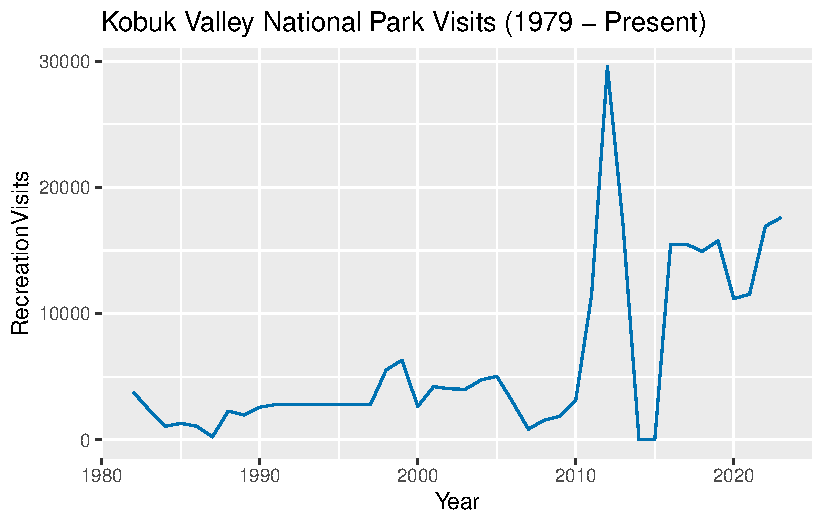
\includegraphics{data-essay_files/figure-pdf/unnamed-chunk-9-1.pdf}

But it turns out that in 2014 and 2015, Kobuk Valley National Park
actually didn't count visitors at all.

If we look at the
\href{https://irma.nps.gov/Stats/SSRSReports/Park\%20Specific\%20Reports/Monthly\%20Visitation\%20Comments\%20By\%20Park?Park=KOVA}{visitation
reports for Kobuk Valley in 2014}, they say that ``the park is
developing a new counting system and has made the decision not to report
visitor counts until the new system is in place.'' But even though they
didn't count visitors at all, they still recorded a zero in those two
years. This hard number makes it seem conclusive, like there really were
zero people people who stepped onto the park lands in those years.

In 2015, John Quinley, the Alaska regional spokesperson for the NPS,
spoke with the Anchorage Daily News about this issue, and he admitted
that ``it might have been better if park statisticians had put something
other than a zero in the visitor box for 2014 --- say maybe a question
mark.''

\begin{tcolorbox}[enhanced jigsaw, bottomrule=.15mm, colback=white, colbacktitle=quarto-callout-tip-color!10!white, coltitle=black, titlerule=0mm, leftrule=.75mm, toprule=.15mm, opacitybacktitle=0.6, colframe=quarto-callout-tip-color-frame, opacityback=0, rightrule=.15mm, breakable, bottomtitle=1mm, toptitle=1mm, title=\textcolor{quarto-callout-tip-color}{\faLightbulb}\hspace{0.5em}{Discussion}, left=2mm, arc=.35mm]

Why would you or wouldn't you want to record a question mark in this
dataset? What else could you use to record uncertainty?

\end{tcolorbox}

The decision not to record visits in certain years seems reasonable on
its face, but we've also seen a \emph{lot} of parks in more
highly-frequented areas that, when faced with a similar situation, chose
to provide an estimate for a certain year based on average counts from
previous years, rather than simply declare that nobody visited. This
matters because, as we've discussed, there are financial, political, and
social ramifications of these visit count numbers.

\subsection{Conclusion}\label{conclusion}

To-do

\subsection{References}\label{references}

\phantomsection\label{refs}
\begin{CSLReferences}{1}{0}
\bibitem[\citeproctext]{ref-alba_covid-19s_2022}
Alba, Charles, Bing Pan, Junjun Yin, William L. Rice, Prasenjit Mitra,
Michael S. Lin, and Yun Liang. 2022. {``{COVID}-19's Impact on
Visitation Behavior to {US} National Parks from Communities of Color:
Evidence from Mobile Phone Data.''} \emph{Scientific Reports} 12 (1):
13398. \url{https://doi.org/10.1038/s41598-022-16330-z}.

\bibitem[\citeproctext]{ref-beauchamp_beyond_2020}
Beauchamp, Toby. 2020. {``Beyond the {`{Pine} {Pig}'}: {Reimagining}
{Protection} Through the {US} {National} {Park} {Ranger}.''}
\emph{Radical History Review} 2020 (137): 96--118.
\url{https://doi.org/10.1215/01636545-8092798}.

\bibitem[\citeproctext]{ref-floyd_coming_2002}
Floyd, Myron F., and Cassandra Y. Johnson. 2002. {``Coming to {Terms}
with {Environmental} {Justice} in {Outdoor} {Recreation}: {A}
{Conceptual} {Discussion} with {Research} {Implications}.''}
\emph{Leisure Sciences}, January.
\url{https://doi.org/10.1080/01490400252772836}.

\bibitem[\citeproctext]{ref-weber_why_2013}
Weber, Joe, and Selima Sultana. 2013. {``Why {Do} {So} {Few} {Minority}
{People} {Visit} {National} {Parks}? {Visitation} and the
{Accessibility} of {`{America}'s {Best} {Idea}'}.''} \emph{Annals of the
Association of American Geographers} 103 (3): 437--64.
\url{https://doi.org/10.1080/00045608.2012.689240}.

\end{CSLReferences}

\section{Explore the Data}\label{tabset-1-2}

\begin{Shaded}
\begin{Highlighting}[]
\NormalTok{//| echo: false}
\NormalTok{//| output: false}
\NormalTok{visit\_data = d3.csv("https://raw.githubusercontent.com/melaniewalsh/responsible{-}datasets{-}in{-}context/main/datasets/national{-}parks/US{-}National{-}Parks\_RecreationVisits\_1979{-}2023.csv", d3.autoType)}

\NormalTok{use\_data = d3.csv("https://raw.githubusercontent.com/melaniewalsh/responsible{-}datasets{-}in{-}context/main/datasets/national{-}parks/US{-}National{-}Parks\_Use\_1979{-}2023\_By{-}Month.csv", d3.autoType)}
\end{Highlighting}
\end{Shaded}

\begin{Shaded}
\begin{Highlighting}[]
\NormalTok{//| echo: false}
\NormalTok{//| output: false}


\NormalTok{filtered = visit\_data.filter(function(penguin) \{}
\NormalTok{  return bill\_length\_min \textless{} penguin.bill\_length\_mm \&\&}
\NormalTok{         islands.includes(penguin.island);}
\NormalTok{\})}
\end{Highlighting}
\end{Shaded}

\begin{Shaded}
\begin{Highlighting}[]
\NormalTok{//| echo: false}
\NormalTok{color = d3}
\NormalTok{  .scaleLinear()}
\NormalTok{  .domain([5000000, 1000000, 100000])}
\NormalTok{  .range(["\#cafcc2", "\#fce7c2", "\#eb9494"])}
\end{Highlighting}
\end{Shaded}

\subsection{U.S. National Park Visits
---~1979-2023}\label{u.s.-national-park-visits-1979-2023}

\begin{Shaded}
\begin{Highlighting}[]
\NormalTok{//| echo: false}
\NormalTok{viewof search = Inputs.search(visit\_data, \{}
\NormalTok{  placeholder: "Search"}
\NormalTok{\})}
\end{Highlighting}
\end{Shaded}

\begin{Shaded}
\begin{Highlighting}[]
\NormalTok{//| echo: false}

\NormalTok{/*Inputs.table(search, data)*/}

\NormalTok{Inputs.table(search, \{}
\NormalTok{  layout: "fixed",}
\NormalTok{  rows: 50,}
\NormalTok{  sort: "Year",}
\NormalTok{  reverse: true,}
\NormalTok{  format: \{}
\NormalTok{    /*RecreationVisits: x =\textgreater{} d3.format(\textquotesingle{}.2s\textquotesingle{})(x),*/}
\NormalTok{    Year: x =\textgreater{} d3.timeFormat(x),}
\NormalTok{    RecreationVisits: x =\textgreater{} html\textasciigrave{}\textless{}div style=\textquotesingle{}background:$\{color(x)\}\textquotesingle{}\textgreater{}$\{d3.format(\textquotesingle{}.2s\textquotesingle{})(x)\}\textless{}/div\textgreater{}\textasciigrave{}}
\NormalTok{  \}}
\NormalTok{\})}
\end{Highlighting}
\end{Shaded}

\subsection{U.S. National Park Use (Monthly)
---~1979-2023}\label{u.s.-national-park-use-monthly-1979-2023}

\begin{Shaded}
\begin{Highlighting}[]
\NormalTok{//| echo: false}
\NormalTok{viewof use\_search = Inputs.search(use\_data, \{}
\NormalTok{  placeholder: "Search"}
\NormalTok{\})}
\end{Highlighting}
\end{Shaded}

\begin{Shaded}
\begin{Highlighting}[]
\NormalTok{//| echo: false}

\NormalTok{/*Inputs.table(search, data)*/}

\NormalTok{Inputs.table(use\_search, \{}
\NormalTok{  layout: "fixed",}
\NormalTok{  rows: 50,}
\NormalTok{  sort: "Year",}
\NormalTok{  reverse: true,}
\NormalTok{  format: \{}
\NormalTok{    /*RecreationVisits: x =\textgreater{} d3.format(\textquotesingle{}.2s\textquotesingle{})(x),*/}
\NormalTok{    Year: x =\textgreater{} d3.timeFormat(x),}
\NormalTok{    RecreationVisits: x =\textgreater{} html\textasciigrave{}\textless{}div style=\textquotesingle{}background:$\{color(x)\}\textquotesingle{}\textgreater{}$\{d3.format(\textquotesingle{}.2s\textquotesingle{})(x)\}\textless{}/div\textgreater{}\textasciigrave{}}
\NormalTok{  \}}
\NormalTok{\})}
\end{Highlighting}
\end{Shaded}

\section{Exercises}\label{exercises}

\section{R}

\phantomsection\label{exercise-posts}

\section{Python}

\section{Discussion \& Activities}\label{discussion-and-activities}

\subsection{Activity 1}\label{activity-1-1}

It is inevitable that the devices that the National Park Service uses to
count visits to the parks ---~like induction loop counters installed on
the road ---~will break. But they will also get \emph{fixed} at
different rates, in different locations, as we could see in the case of
Crater Lake National Park (where a counter was fixed quickly) and
Carlsbad Caverns National Park (where a broken counter from 2019 still
has not been fixed).

There are many reasons for these disparities, but some of the big ones
might be geography and resources. The more remote a park, the harder it
is to get a repair team to it. The less-resourced a park, the lower the
likelihood they have on-site repair teams, or are prioritized by the
repair teams that can be dispatched.

With this in mind, look at the locations of the following parks. Suppose
that each one has an outage in their induction loop counter: which ones
would you expect to be fixed first, and why? Research the parks, and
rank them on a scale of 1 to 5 (1 being highest, and 5 being lowest) of
which would be fixed quickest.

\begin{longtable}[]{@{}lll@{}}
\toprule\noalign{}
Park & Priority (1-5) & Reason \\
\midrule\noalign{}
\endhead
\bottomrule\noalign{}
\endlastfoot
Acadia NP & & \\
Lassen Volcanic NP & & \\
Saguaro NP & & \\
Yosemite NP & & \\
Mammoth Cave NP & & \\
\end{longtable}

\subsection{Activity 2}\label{activity-2}

The National Park Service sometimes fills in missing data with hard
numbers or approximates data by applying special mathematical formulas.
This is necessary work, but it is also under-explained work.

To see this in action, go to
\href{https://irma.nps.gov/Stats/Reports/Park}{the NPS page that
documents park reports} and down the ``Visitor Use Counting Procedures''
PDF for three different parks.

How are the procedures for these three parks similar or different? What
kind of effect do you think this has on the resulting data? What do you
think is the best of documenting this information and communicating it
to users of the data?

\subsection{Activity 3}\label{activity-3}

In 2014 and 2015, Kobuk Valley National Park reported that there were
zero visitors to the park.

Use publicly available internet data - Twitter posts, Flickr photos, etc
- to try and find evidence of people visiting the park (there is
existing evidence!).

Based on your findings, how do you think, differently, if at all, about
Kobuk Valley's decision to record zero visits and about alternative
methods for counting visits?

:::



\end{document}
